\chapter{Gestão de configuração de software}
\label{cap-referencial}

De acordo com \citeonline{ieegcs}, gestão de configuração de software \textit{(GCS)} 
é uma área da engenharia de software cujo objetivo é:

\begin{itemize}
  \item Identificar e documentar as características funcionais de
  um produto.
  \item Controlar quaisquer alterações a estas características.
  \item Registrar e relatar cada mudança do seu estágio de implantação
  \item Apoiar a auditoria dos produtos, resultados, serviços ou
componentes para verificar a conformidade com requisitos

\end{itemize}

Gestão de Configuração de Software é uma das capacidades fundamentais que devem
estar em qualquer projeto de desenvolvimento de software. Ela é
tradicionalmente dividida em três atividades, e são elas: configuração,
identificação e controle. Isto é encarado como uma ferramenta de
gestão que pode ajudar na orientação de cada projeto, pois ajuda a manter a
integridade do produto e manter a qualidade do projeto sob controle \cite{gcs}. 

Ela também é essencial para a engenharia de software, pois estabelece e protege a
integridade de um produto ao longo da sua vida útil, percorrendo através dos
processos de desenvolvimento, teste e entrega do produto, bem como
durante a sua instalação, operação, manutenção e eventual evolução \cite{ieegcs}.

Gestão de configuração de software também fornece a infraestrutura que é a base para
qualquer tipo de projeto de software. Isto facilita a coordenação e comunicação
entre os vários participantes numa equipe de desenvolvimento de software.
Dentro da gestão de configuração de software
existem várias áreas de atuação \cite{gcs}. Este trabalho aborda especificamente a 
implantação de software.

Este capítulo possui a Seção \ref{sec:implantacao}, que fala sobre
implantação de software, além da Seção \ref{subsec:DevOps} que fala sobre 
\textit{DevOps}, uma
nova abordagem que traz um conceito de implantação
automatizada de software junto aos métodos ágeis de desenvolvimento de software. 

Depois, a Seção \ref{subsec:metodoseferramentas} que fala sobre
ferramentas e técnicas que buscam facilitar e resolver os problemas da
implantação automatizada de software.

E por fim, a Seção \ref{sec:seguranca}, que fala sobre quais são os procedimentos 
que devem ser levados em consideração durante uma implantação de aplicações voltada
para a web.

\section{Implantação de Software}
\label{sec:implantacao}
Software só oferece valor para os clientes quando ele está implantado e em produção,
e assim, possa proporcionar as funcionalidades necessárias ao usuário final. Por
 isso, a importância da fase de implantação de software, pois é nessa fase em que a equipe
de desenvolvimento disponibilizará o software ou uma atualização com novas funcionalidades
ao usuário. 

Sendo assim, a implantação de software é um conjunto de atividades cruciais
para todos os fornecedores de software. Isto começa desde um pedido de um novo requisito
de software, até todas as medidas necessárias para que essa nova versão fique disponível
para o cliente \cite{5741269}. A implantação de software é composta por várias
atividades que são essenciais para disponibilizar um produto a alguém, como por exemplo:
instalação de dependências, arquivos de configuração e instalação da própria aplicação.

Uma grande aliada das equipes de desenvolvimento é a implantação automatizada de
software, que se refere à prática de implantar o software para os usuários finais
automaticamente, evitando qualquer tipo de execução de esforço manual. Por isso,
a prática de implantação automatizada facilita na rápida entrega de software, tanto
para implantações de aplicações em servidores na nuvem, como implantação de software
para usuários em seus computadores \cite{7284592}.

As aplicações de software não são mais sistemas isolados, 
são cada vez mais o resultado da integração de coleções de
componentes. Isso pode tornar a implantação de software um processo complicado, e
nem sempre existir a garantia de que cada componente será implantado corretamente.
Portanto, a equipe de desenvolvimento deve encontrar uma maneira de lidar
com uma maior incerteza no ambiente nos quais seus sistemas vão operar, garantindo
que a implantação do software seja feita da forma correta, evitando qualquer acontecimento
de erros e imprevistos \cite{deployment1998}.

\subsection{Processo de Implantação de Software}
\label{sub:processoimplantacao}

A implantação de um software é o processo que vai desde a aquisição desse software
até a sua execução \cite{leo2014}.

A Object Management Group \textit{(OMG)} é uma organização internacional sem fins lucrativos,
que aprova padrões abertos para tecnologias. Eles definem uma especificação de
implantação e configuração de aplicações distribuídas baseadas em componentes \cite{omg2006}. 
A \textit{OMG} também diz que o processo de implantação é um processo que se inicia desde
a aquisição de um componente, até o momento em que esse componente está em plena
execução pronto pra uso.

Segundo \citeonline{omg2006} os principais termos definidos dentro de uma implantação
de software são:

\begin{itemize}
  \item  \textbf{Implantador:} Pessoa ou equipe responsável pelo processo de
  implantação  de um sistema.
  \item  \textbf{Ambiente alvo:} São o servidor ou conjunto de servidores em
  que os componentes são implantados.
  \item  \textbf{Nó:} É um recurso computacional onde se implanta um componente,
  por exemplo uma máquina virtual dentro do servidor que vai hospedar um serviço
  de banco de dados. Os nós fazem parte do ambiente alvo.
  \item  \textbf{Pacote:} Artefato executável que contém o código binário do componente ou código
fonte pronto para instalação ou compilação. É por meio de um pacote que um serviço pode ser instalado e executado dentro
  de um sistema operacional, e que são característicos dependendo da distribuição
  do sistema operacional, por exemplo: .deb para Debian e .rpm para Redhat, ou
  pacotes independentes de sistema operacional como por exemplo pacotes Jar para java,
pacotes Pip para o python e Gem para ruby.
\end{itemize}

Além disso, são definidas as fases que compõem o processo de implantação e de acordo
com \citeonline{omg2006} as fases são:

\begin{itemize}
  \item  \textbf{Planejamento:} O planejamento da implantação é uma fase
  para identificar os componentes necessários na implantação e como cada um será
  distribuído entre os nós do ambiente alvo.
  \item  \textbf{Preparação:} São os procedimentos necessários para preparar o
  ambiente alvo para que um determinado componente possa ser executado, isso envolve
  configuração do sistema operacional, instalação e configuração de dependências
  necessárias (por exemplo um servidor web como Apache ou Nginx). 
  \item  \textbf{Instalação:} O implantador transfere o componente para a infraestrutura
  alvo, é quando instalamos um dado componente em um servidor, um exemplo disso
  é a instalação de uma aplicação via pacotes (.deb ou .rpm).
  \item  \textbf{Configuração:} Edição de arquivos de configuração para alterar
  determinado comportamento de uma aplicação, o implantador aplica configurações
  específicas à aplicação a partir de arquivos de configuração.
  \item  \textbf{Inicialização:} É quando a aplicação é iniciada e entra em execução,
  pronta para receber chamadas de seus clientes.
\end{itemize}

Os termos e fases formam uma estrutura básica que um processo de implantação de software
deve conter. Cada fase é necessária para que se possa ter uma implantação consistente, ou seja, as
atividades dentro de uma implantação de software estarão organizadas, evitando assim
possíveis erros durante a implantação. Essa organização também pode ajudar os 
implantadores a diagnosticar eventuais problemas.

Dependendo do tamanho da aplicação as fases podem se tornar tarefas complicadas,
por isso, existe a necessidade de automatizar o processo de implantação. Isso 
diminui a possibilidade de erros, comparado a uma tarefa manual, e consequentemente
torna o trabalho mais ágil, eliminando a necessidade de manuais de instalação. 
O objetivo de um processo de implantação automatizado é proporcionar uma implantação confiável e 
fácil de ser executada \cite{humble2010}.

Para que a implantação automatizada de software seja possível, é necessário o uso
de ferramentas que possam automatizar todo o processo de implantação. Porém, é 
necessário que o implantador compreenda cada fase do processo para que possa ser
feito um bom planejamento e execução da implantação.

\section{Desenvolvimento e Operações (DevOps)}
\label{subsec:DevOps}
Como resultado ao longo dos anos, as equipes de desenvolvimento de software
são capazes de entregar software a um ritmo muito mais rápido, principalmente com a adoção
de métodos ágeis de desenvolvimento de software \cite{7173368}. As 
equipes desenvolvem de forma acelerada, enquanto a equipe de operações consegue 
implantar software de forma sequencial. Sendo assim, \textit{DevOps}
nasceu a partir dessa necessidade, de implantar software no mesmo ritmo em que
as equipes são capazes de entregar novas funcionalidades.

\textit{DevOps} pode ser visto como um conjunto de práticas e princípios para a 
entrega de software, com foco na velocidade de entrega e na automação \cite{7173368}. 
Antes o time de desenvolvimento terminava suas funcionalidades e seus testes e
entregava a uma equipe de implantação, e a equipe de implantação precisava
lidar com os problemas sem a ajuda do time de desenvolvimento. Por isso \textit{DevOps} 
tenta unir esses dois mundos, fazendo com que as duas equipes compartilhem atividades
 e responsabilidades \cite{6265084}.

A comunidade \textit{DevOps} defende a comunicação
entre a equipe de operações e a equipe de desenvolvimento, como um meio de assegurar
que o os desenvolvedores entendam os problemas associados com as operações. Um dos
principais benefícios disso, é a capacidade de quantificar os problemas dos dois mundos,
para que possa levar a melhoria do desenvolvimento do produto \cite{httermann2012DevOps}.

Em \citeonline{7173368} são abordados as práticas \textit{DevOps}, que podem ser 
aplicadas diversas vezes dentro de um ciclo de desenvolvimento de software. As 
praticas \textit{DevOps} podem ser resumidas em:

 \begin{itemize}
   \item \textbf{Planejamento Contínuo:} O planejamento da equipe de operações 
deve ser sempre contínuo
   e evoluído junto ao planejamento da equipe de desenvolvimento, com tarefas
   sendo priorizadas o tempo todo e sempre alinhadas de acordo com as decisões tomadas
   em conjunto com a equipe de desenvolvimento.
   \item \textbf{Integração Contínua:} Compartilhar as alterações feitas com toda equipe
   evitando que as novas modificações fiquem apenas nas mãos do time de desenvolvimento.
   \item \textbf{Implantação Contínua:} O coração do \textit{DevOps}, recomenda-se automatizar
   todo o processo de implantação, removendo qualquer tipo de etapas manuais com auxílio
   de uma ferramenta que possa automatizar a instalação, sendo assim a implantação
   de cada nova versão de software passa a ser feita de forma mais rápida e eficiente.
   \item \textbf{Testes Contínuos:} Automatiza também os testes da sua aplicação.
   \item \textbf{Monitoração Contínua:} Monitorar as novas alterações
   que foram implantadas a fim de aumentar a capacidade de reagir a quaisquer surpresas
   em tempo hábil.
 \end{itemize}

Os benefícios do uso do \textit{DevOps} são vários, como por exemplo: economia de tempo,
já que implantação de software passa a ser um processo natural e automatizado, 
gerando economia de custos, e aumentando a eficiência do desenvolvimento de software como um todo \cite{7173368}.

Nesse trabalho, foi utilizada a prática \textit{DevOps} de implantação contínua,
automatizando todo o processo de implantação de aplicações web. 

Para entender melhor a prática de implantação automatizada, que é o coração
do \textit{DevOps}, na Subseção \ref{subsub:infracode} será abordado a infraestrutura
como código, que é uma prática bastante difundida nas comunidades \textit{DevOps}.

\subsection{Infraestrutura como código}
\label{subsub:infracode}
Infraestrutura como código é a prática de especificar configurações de
sistema de computação através de código, com o intuito de automatizar a implantação
de um software e o seu gerenciamento de configurações. Por exemplo, um sistema
com diferentes configurações de hardware e diferentes
requisitos de software podem ser especificados e implantados automaticamente
sem intervenção humana \cite{configurationcodesmell}. 

Tal procedimento pode ser
ainda personalizado, conforme as necessidades da implantação. Sendo assim, a implantação
automatizada não só é mais rápida do que o processo manual, mas também é mais
confiável e reproduzível.

Para aplicar a infraestrutura como código em um projeto, é necessário
migrar a infraestrutura do projeto em código, essencialmente como um
código que o desenvolvedor lida no seu trabalho diário \cite{byhand}.

Dado que um \textit{script} de configuração realmente contém código, é mais natural
para o desenvolvedor tratá-lo como tal, utilizando suas habilidades de codificação,
além de poder utilizar ferramentas que auxiliem a prática do \textit{DevOps} e de colaboração,
entre a equipe de desenvolvimento e a equipe de infraestrutura \cite{byhand}. 

Com a infraestrutura sendo tratada como código, é possível utilizar um
sistema de controle de versão que permita outras pessoas colaborem e trabalhem em
equipe. Com a ajuda de um sistema de controle de versão, por exemplo, é possível 
ter uma documentação completa do estado do seu sistema, 
através do histórico de alterações, para que seja possível
trazer o código da infraestrutura para um estado desejado a partir de
qualquer outro estado.

Para realizar essa prática, existem ferramentas como Chef \footnote{https://www.chef.io/chef/} e 
Puppet \footnote{https://puppet.com/}, que
fornecem aos desenvolvedores várias abstrações para 
expressar etapas de automação,
de forma independente. Esses recursos podem ser executados várias vezes,
obtendo-se sempre o mesmo resultado, trazendo uma capacidade de atingir um determinado
estado desejado. Isso permite múltiplas iterações, 
com implantações frequentes de infraestruturas complexas
\cite{Hummer2013}.

\section{Métodos e ferramentas para implantação automatizada de software}
\label{subsec:metodoseferramentas}

Existem várias soluções técnicas para melhorar a implantação de software. No 
entanto, apesar da sua importância para as empresas de software, as atividades
de implantação de software têm recebido pouca atenção \cite{5741269}. Recentemente 
um número de novas tecnologias começaram a emergir para
resolver o problema de implantação. As características típicas oferecidas por
estas tecnologias incluem sistemas para automatizar a implantação a partir de
configurações, pacotes, gerenciamento de rede e instalação de recursos, com
propósito de entrega das atualizações de forma automática \cite{deployment1998}.

Para a implantação automatizada de software, é
possível utilizar linguagens de \textit{script} de propósito
geral como: Python, Ruby e Shellscript. Também existem ferramentas gerais 
voltadas para o processo de implantação, como sistemas de \textit{middleware} 
especializados em determinados tipos de artefatos implantáveis \cite{leo2014}.

Um processo de implantação automatizado depende bastante da integração de diferentes papéis
numa organização. Como foi dito na Seção \ref{subsec:DevOps}, é importante a
integração entre desenvolvedores e operadores, uma vez que o desenvolvimento desses
\textit{scripts} ou utilização das ferramentas precisam de participação de ambos os perfis.

Tais ferramentas, permitem-nos controlar e automatizar a configuração de todos os 
elementos que compõem um sistema. São eles: software a serem instalados,
usuários do sistema, serviços em execução, arquivos de configuração, tarefas agendadas,
configuração de rede, armazenamento de arquivos, monitoramento e segurança. A sua 
função principal é automatizar a instalação e configuração de um 
sistema. 

Com essas ferramentas, é possível escrever algumas regras que expressam como 
um software deve ser configurado, e assim, a ferramenta configurará o sistema conforme as 
especificações. Essas ferramentas funcionam de forma declarativa, 
especificando a instalação de um software através de regras \cite{6265084}.

Por exemplo, é possível especificar regras para a configuração do sistema
a partir de uma infraestrutura básica. No Chef, essa estrutura é conhecida como livro
de receitas, já em Puppet, essa estrutura é conhecida como manifesto. Esses recursos
são basicamente arquivos, no qual o implantador define os passos que serão executados. 

Cada passo da configuração desejada pode depender de outros passos, ou seja, para
instalar uma aplicação pode ser necessário instalar previamente um compilador ou interpretador
 da linguagem. Um outro exemplo é que para executar uma aplicação web é necessário a 
instalação prévia de um servidor web. Para lidar com as dependências essas 
ferramentas descrevem o estado em que a aplicação deve estar, ou seja, 
todos os pacotes, arquivos de configuração diretórios e usuários, sendo possível 
definir a dependência entre as tarefas a serem executadas.

Com essas ferramentas a implantação de um software dentro de uma infraestrutura
não precisa de esforço manual. Com elas, é possível automatizar toda a implantação
de um software, desde a preparação do ambiente até a inicialização da aplicação. 
Sendo assim, reduzir o tempo gasto na implantação sem qualquer esforço
adicional.

Além das ferramentas de automação, é importante também entender o empacotamento de
programas. Tanto Chef como Puppet utilizam a instalação de pacotes como recurso para
poder instalar softwares, ou seja, é possível buscar os softwares desejados a partir
dos pacotes disponíveis numa distribuição GNU/Linux. 

As distribuições GNU/Linux que
optam por disponibilizar pacotes, mantém uma infraestrutura de servidores como fonte
de distribuição de programas \cite{araujo2011apprecommender}. Tais servidores são
chamados de repositórios, e esses pacotes são gerenciados com softwares conhecidos
como sistemas gerenciadores de pacotes, que possuem a responsabilidade de buscar
os softwares a serem instalados que estão disponíveis nos respectivos repositórios.

\subsection{Pacotes Debian}

O formato utilizado pelo Debian GNU/Linux e seus derivados é o formato de pacotes
binários conhecido como .deb. Um pacote .deb é composto de arquivos executáveis,
bibliotecas e documentação associada a um programa ou a um conjunto de programas,
além de todos os dados e procedimentos necessários para instalar, configurar e remover
aplicativos de um sistema \cite{araujo2011apprecommender}. A estrutura dos pacotes 
.deb e seus requisitos para que sejam distribuídos oficialmente pelo Debian,
estão especificados no Manual de Políticas do Debian \cite{debian}.

Ao instalar um pacote .deb, são feitos todos os procedimentos necessários para a instalação
de uma aplicação, porém, existem ainda, casos em que o usuário precise fazer
configurações adicionais. Um exemplo é quando o usuário precisa configurar um banco de dados
ou fazer uma configuração específica de uma aplicação a partir de arquivos de configuração.

Essas tarefas não são de responsabilidade dos pacotes, e sim do usuário que deseja utilizar esse
software, já que o pacote não poderia prever qual é a estrutura e a configuração
que o usuário pretende utilizar. Logo, a execução desses passos é feita de
acordo com a preferência do usuário, podendo ser feita manualmente ou a partir
de uma implantação automatizada que utilize alguma ferramenta para isso. Um exemplo
desse tipo de atividade, que não é de responsabilidade de um pacote, é a configuração
de hospedagem virtual, que será visto na Subseção \ref{sub:multiplas}.

\subsection{Múltiplas Instâncias de Aplicações Web com Hospedagem Virtual}
\label{sub:multiplas}
Na implantação de software, é necessário escolher um ambiente alvo, onde a aplicação
será instalada. Esse ambiente deve possuir um nó, que é um recurso computacional
onde se implanta um componente. 

Porém, pode existir a necessidade de implantar várias aplicações no mesmo servidor, e no caso
de aplicações web, isso pode ser um problema. O problema é que as aplicações estarão em um
único servidor, assim também em um único endereço de \textit{IP}, e isso pode gerar
conflitos de nomes, visto que nesse caso, todos os serviços precisariam ter o mesmo
nome, e isso seria inviável para várias aplicações no mesmo servidor.

Uma forma de solucionar esse problema é o uso de hospedagem virtual, que é um 
termo que se refere à prática de executar mais de uma aplicação web numa única 
máquina \cite{apachvh}. Com a hospedagem virtual, é possível
hospedar mais de um nome de domínio no mesmo computador, o que possibilita ter
vários nomes de domínio em execução, num único endereço de \textit{IP}. Isso
possibilita que, num mesmo servidor, tenha uma aplicação com o endereço
 www.blog.com e uma outra aplicação com o endereço www.nuvem.com. 

O fato de que eles estão em execução no mesmo servidor físico não é aparente 
para o usuário final. Essa solução é importante para economizar recursos, 
já que não será necessário possuir um servidor dedicado apenas a uma aplicação.

Alguns softwares possuem suporte para a implementação de hospedagem virtual, como por
exemplo o Apache e o Nginx. Além disso, existem vários
outros recursos que essas ferramentas possuem, como por exemplo o recurso de proxy.
Porém, para este trabalho será necessário apenas o uso de hospedagem virtual.

Um resumo do funcionamento de múltiplas instâncias está na Figura \ref{multipla}
\begin{figure}[h]                                                                                                                      
  \centering                                                                    
  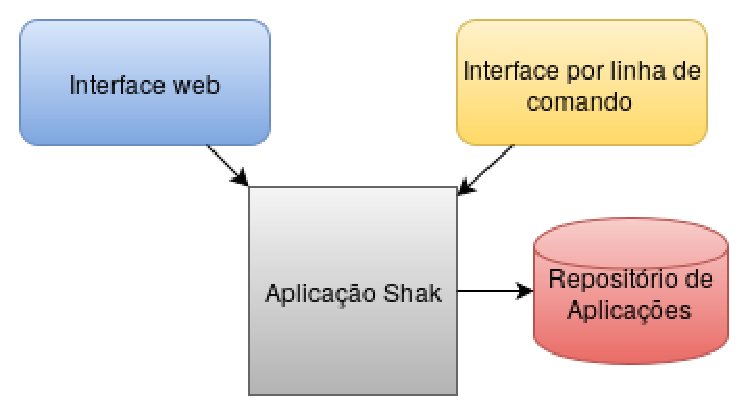
\includegraphics[width=0.5\textwidth]                                         
      {figuras/shak}                                                            
      \caption{Funcionamento de Múltiplas instâncias}                     
  \label{multipla}                                                              
\end{figure} 

\section{Segurança na Implantação de Aplicações Web}
\label{sec:seguranca}

Um pacote cumpre bem suas responsabilidades dentro de uma implantação de
software, porém, outras atividades também são importantes e fogem da responsabilidade 
de um pacote. Outro fator, é que um pacote também não pode prever quais são
os procedimentos de segurança que devem ser tomados numa implantação, como por 
exemplo, a criação de certificados digitais. 

Esses procedimentos estão relacionados à segurança na implantação de aplicações web 
utilizando pacotes Debian, no qual trata o uso de protocolos que utilizam criptografia
para a segurança de dados.

Existem algumas categorias predominantes e prejudiciais de ataques na Internet. São elas: 
ataques via malware, recusa de serviços, analisador
de pacotes, disfarce na fonte e modificação ou exclusão de mensagem. Para proteger
desses ataques é importante o uso de comunicação segura, protegendo as aplicações 
\cite{kurose2010redes} 

Para isso, \citeonline{kurose2010redes} ainda identifica as propriedades 
desejáveis da comunicação segura, sendo elas:

\begin{itemize}
  \item \textbf{Confidencialidade:} Diz respeito a somente o remetente e o destinatário
  pretendido poderem entender o conteúdo da mensagem transmitida.
  \item \textbf{Autenticação do ponto final:} Diz respeito a tanto o remetente como o destinatário
  precisar confirmar a identidade da outra parte envolvida na comunicação.
  \item \textbf{Integridade da Mensagem:} Diz respeito a assegurar que o conteúdo
  da mensagem não seja modificado.
  \item \textbf{Segurança Operacional:} Diz respeito à segurança da rede, no qual
  os atacantes podem tentar adquirir os segredos da rede e lançar ataques DoS,
  por isso é necessário uma boa configuração de firewall e sistemas de detecção
  de invasão.
\end{itemize}

No contexto de implantação de aplicações web, foi tomado como objetivo a segurança
dos dados transmitidos. Com isso, aplicando criptografia nos protocolos da camada
de aplicação, que serão utilizados neste trabalho, sendo eles os protocolos 
Hypertext Transfer Protocol \textit{(HTTP)} e Simple Mail Transfer Protocol 
\textit{(SMTP)}, assim adiciona-se uma camada de segurança nas aplicações que serão implantadas.

\subsection{Protocolos da Camada de Aplicação e Camada de Segurança}

As aplicações web utilizam protocolos da camada de aplicação \cite{kurose2010redes}. 
A camada de aplicação é onde residem as 
aplicações de rede e seus protocolos, incluindo os protocolos \textit{HTTP} e 
\textit{SMTP}, que são protocolos importantes neste trabalho, já que 
aplicações web utilizam o \textit{HTTP} para transferência de arquivos e o \textit{SMTP} para
transferência de mensagens de correio eletrônico. 

Os protocolos \textit{HTTP} e \textit{SMTP} estão especificados em \textit{Request for Comments} 
\textit{(RFC)}, que são documentos técnicos que especifica os padrões implementados
na internet. A 
especificação do protocolo \textit{HTTP} está disponível na \textit{RFC} 2616 
\footnote{https://www.ietf.org/rfc/rfc2616.txt}, já o protocolo \textit{SMTP} 
está especificado na \textit{RFC} 5321 \footnote{https://www.ietf.org/rfc/rfc5321.txt}.

As aplicações que serão utilizadas neste trabalho, são aplicações web empacotadas no
Debian. Aplicações web costumam ser aplicações cliente-servidor, que permitem aos
usuários obterem documentos de servidores web a partir de requisições. Esses documentos 
são padronizados, como por exemplo o \textit{HyperText Markup Language} \textit{HTML}, 
para que os navegadores possam interpretar e passar a informação ao usuário 
\cite{kurose2010redes}.

O \textit{HTTP} é 
implementado em dois programas, um cliente e um servidor, conversando um 
com outro a partir de troca de mensagens. O papel do \textit{HTTP} é definir a 
estrutura dessas mensagens e o modo como o servidor e o cliente as trocam. O 
principal conteúdo das mensagens trocadas entre clientes e servidores são os 
objetos. Um objeto é basicamente um arquivo, podendo ser um vídeo, uma imagem 
ou um arquivo \textit{HTML} \cite{kurose2010redes}.

Já o \textit{SMTP}, é o protocolo responsável por transferir mensagens de servidores de correio
remetentes para servidores de correio destinatários, também transferindo arquivos,
de um servidor de correio para o outro. Uma diferença entre o \textit{HTTP} e o \textit{SMTP}
é que o protocolo \textit{HTTP} é um protocolo de recuperação de informações, enquanto
o protocolo \textit{SMTP} é um protocolo de envio de informações \cite{kurose2010redes}. 

Isso implica que, para um usuário recuperar as informações de e-mail, é necessário 
o uso de outros componentes. Já que isso não é possível via \textit{SMTP}, para 
resolver isto existem os protocolos de acesso ao correio, entre eles o 
\textit{Post Office Protocol} \textit{(POP3)} e \textit{Internet Message Access Protocol} \textit{(IMAP)}.

Para adicionar uma camada de segurança, com sigilo e integridade de dados, é necessário
o uso de outro protocolo, o protocolo \textit{Secure Socket Layer} \textit{(SSL)}, para 
complementar os protocolos \textit{HTTP} e \textit{SMTP}. O protocolo \textit{SSL} 
é utilizado por basicamente todos os sites conhecidos, como Google,
Amazon e eBay. Seu uso é para oferecer segurança em transações, pois ele cria um
canal criptografado entre um servidor e um cliente, garantido que todos os
dados transmitidos sejam sigilosos e seguros \cite{kurose2010redes}. 

Para poder utilizar o \textit{SSL}, é necessário que o servidor 
possua um certificado digital, que possa responder algumas questões sobre a 
identidade do seu servidor. Com as devidas configurações, tanto \textit{HTTP} como 
\textit{SMTP} estarão sobre uma camada adicional de segurança, que utiliza o 
protocolo \textit{SSL}. Essa camada adicional permite que os dados sejam 
transmitidos por meio de uma conexão criptografada e que se verifique a autenticidade
do servidor e do cliente por meio de certificados digitais. 

\subsection{Assinaturas e Certificados Digitais}

As assinaturas e certificados digitais servem para agregar confiança e segurança
nas trocas de dados pela Internet, principalmente quando se trata de troca de informações
sigilosas que precisam de uma confiabilidade maior. O que viabiliza a assinatura 
digital é o emprego de criptografia assimétrica ou criptografia de chaves públicas. 

Logo, a assinatura digital deve ser verificável e não falsificável. Uma
aplicação importante de assinaturas digitais é a certificação de chaves públicas,
que certifica que uma chave pública pertence a uma entidade específica \cite{kurose2010redes},
e a certificação de chaves públicas é utilizada no protocolo \textit{SSL}, visto anteriormente.

Uma maneira de se obter o certificado é através de uma entidade conhecida como
entidade certificadora, que é responsável por validar e emitir certificados, e
verifica se uma entidade é realmente quem ela diz ser. Após essa validação, a
entidade certificadora cria um certificado que vincula a chave pública da entidade
a essa verificação, assim o certificado passa a ter a chave pública e a
identificação de que é realmente o proprietário daquela chave pública.

Porém, essas entidades certificadoras cobram por esse serviço, e os certificados também
possuem validade. Uma outra maneira de se obter certificados é a partir dos certificados
autoassinados, que são os certificados gerados por conta própria através de
ferramentas, um exemplo de ferramenta é a ferramenta OpenSSL, que permite requisitar,
assinar, gerar, exportar e converter certificados digitais.

Um problema em utilizar certificados autoassinados é que os clientes, como navegadores,
aceitam apenas os certificados das entidades certificadores em quem eles confiam. Por
exemplo, um navegador não vai conhecer o certificado que foi autoassinado por
alguém que ele não conhece, e logo vai avisar ao usuário de que ele não está numa
conexão segura, por mais que esteja sobre uma conexão \textit{HTTPS}. 

Por isso, 
manter certificados
autoassinados pode gerar esse desconforto, porém é uma saída, principalmente para
fins de testes, e melhor do que não utilizar nenhum tipo de segurança.

Entretanto, em 2014, a Universidade de Michigan e a fundação Mozilla, entre outras 
instituições e empresas, criaram uma nova entidade certificadora, que se chama 
Let's Encrypt, que fornece certificados digitais de forma gratuita, e que são 
reconhecidos por todos os navegadores. Let's Encrypt utiliza o protocolo \textit{ACME} \cite{ACME}, que faz o trabalho de automatizar a validação da identidade pela autoridade 
certificadora, facilitando a configuração de aplicações web com \textit{HTTPS}. 

Este trabalho aborda apenas os certificados autoassinados, porém, o suporte
a certificados que utilizam Let's Encrypt foi referenciado nos trabalhos futuros.
